\documentclass[10pt, final]{article}

\usepackage{./tex_refs/style}

\title{Railway Track Fault Detection\\\large Mathemathical Modeling Practice\\}
\author{Tamás DEMUS\\XP4B9D}
\date{Fall Semester 2022}

\begin{document}
\maketitle
\tableofcontents
\section{Introduction} \label{sec:intro}
Analyzing images and processing the information stored within is a key field of machine learning.
Classification of different images, identifying and localizing different objects are basic problems.
Several real-life cases prove the usability of such approach such as traffic sign recognition,
object detection or face recognition.
The target of current research is to endeavour to create an algorithm that is able to classify images
taken from parts of the rail track to classify whether the rail is defect or not.

A comprehensive overview about visual inspection technologies used in the railway sector is given
in \cite{liu_review_2019}.
It focuses on different technologies including machine learning and non machine learning applications
and covers the overall railway sector including track, vehicle and infrastructure elements.
The following major application categories identified: the railway track, the pantograph-catenary
subsytem, the train body and rail infrastructure.
The railway track is discussed in several subpoints: the detection of rail surface defects, wear and
deformation of track components, identification of rail components and the detection and extraction  of rails.
Current summary follows this review focusing on the track inspection methods applying machine learning
algorithms based on image processing.

\subsection{Surface defect detection}
\citeauthor*{xue_wang_machine-vision_2008} presents a rail surface defect detection method \cite{xue_wang_machine-vision_2008}
based on a liner CCD followed by image processing and applying a Quantum Neural Network (QNN).
The accuracy results were evaluated and compared between QNN, Artifical Neural Network (ANN)
and Support Vector Machine (SVM).
First it detects region of interests (ROI) in the captured images by selecting pixels where the gray-level
quantity is above a certain threshold.
Then it searches for edges to identify the pixels that belong to certain edges.
Then comparing this two set of points, a region of interest is defined by the presence of a set of pixels
in both sets.
Once this are marked, a rectangle can be drawn to enclose the region.
Next step if to extract the features from the single ROIs.
The features are defined based on the geometry of the flaw inside the ROI, the grey-level of the flaw pixels,
and a so-called tansform-space, where a discrete cosine transform filter is applied.
The obtained recalls are ranging between 86.7\% and 100\% depending on the type of flaw.

Another solution for rail surface defect detection is described in \cite{ma_texture_2016}.
Images taken by maintenance vehicles from the top and evaluated for surface defects via two SVM classifiers
applied one after the another.
Overall 8 defect categories differentiated including the non-defect case.
939 manually annotated images was used for the experiments.
A Random Forest based edge detection is followed by a Generalized Hough transform to detect the position of the rails.
This overperformed the Canny edge detection method.
Defect severity level classification was traced back to a texture classification task for that a Bag of Words model
is used.
A set of filters are used to create the feature vectors for each pixel in each image.
From this the dictionary is created via a k-means clustering resulting in a histogram of k bins containing the number
of pixels in each bin.
These descriptors were fed for a $\chi^2$-kernel SVM for training.
Besides the dictionary texton forests were built.
Instead of predicting the class, texton forests predict the image descriptors.
The two methods were combined to an ensemble method by applying stacking.
Overall 5 texton forest SVM classifier and 4 texton dictionary SVM classifier provides 9 probability vector with
8 elements for the 8 classes.
A second level linear-kernel SVM was fitted to these outputs.
An accuracy of 82\% is achieved in the end.

\citeauthor*{santur_new_2017} presents a laser based imaging technology combined with deep learning model \cite{santur_new_2017}.
The rail profile is aquired via laser scanning and afterwards a convolutional neural network is applied.
The article distinguishes between 4 defects: cracks, abrasion, corrugation and headchecks,
however only binary classification is implemented (faulty or not faulty image).
The rail imaging is done via stereovision, time of flight and laser triangulation to obtain a 3d image.
Convolutional Neural Network (CNN) was applied on the image.
The mentioned system achieved 98\% accuracy.

\citeauthor*{li_cyber-enabled_2018} introduces a corrugation identification system that consists of an image
acquisition system and the corresponding machine learning algorithm \cite{li_cyber-enabled_2018}.
The images are taken from the top by equipment fitted to the underframe of the vehicle.
The image processing covers the localization of the rail, feature extraction and corrugation recognition steps.
Rail localization is done on the observation that the rail brightness is high and even and mostly located on the
center of the picture.
Features extracted by applying Fourier transformation for each column (lengthwise part of the rail surface) to
determine the Fourier energy spectrum after truncation and sampling to reduce the dimensionality.
Observation taken that the longitudinal average gray value is relatively high and distributed uniformly.
Corrugation lines represented as periodic changes of the gray value that is a sparse energy distribution
in the frequency domain.
Corrugation afterwards can be detected by an SVM trained on these features.
The proposed solution reaches 99\% accuracy.

\subsection{Component detection}
\citeauthor{li_component-based_2011} presents a methodology in his work in \cite{li_component-based_2011}
extended in \cite{trinh_enhanced_2012} and \cite{ying_li_rail_2014} to detect missing rail components
focusing on the tie plate and it's surrounding localization.
A fixed position camera is used in the research that allows a steady assessment of the track components.
Mostly relying on edge detection methods on grayscale images,
at first detecting the tie plate itself and then the other components can be identified
based on the geometrical positioning.

Connection element binary classification is presented in \cite{mazzeo_visual_2004} that is explained more
in detail in \cite{marino_real-time_2007}.
The method is able to detect the presence of fastener bolts or hooks.
Fastening elements are extracted as features from grayscale pictures taken from top view.
Wavelet transformation and principal component analysis (PCA) performed to describe the features
in low dimensionality.
During the wavelet transformation a high-pass and low-pass filter is applied in every combination,
extended by applying the same combinations on the low-pass-low-pass result.
This results in a multilevel (depending on the number of extensions) wavelet transform.
Two type of neural networks considered: Multilayer Perceptron and Radial Basis Function.
A training set of 173 images used for the bolt detection and 221 images for the hook detection.
Depending on the object to detect the wavelet transformation with levels of 3, 4, and 5 performed best,
reaching accuracy rates of above 98\% in almost all cases.

A commercial solution is presented in \cite{de_ruvo_gpu-based_2009} utilizing GPU based hardware.
It consists of an integrated image acquisition system followed by a prediction modul to identify image areas
for classification and a bolt detection module.
The bolt detection module uses Multilayer Perceptual Network Classifiers (MLPNC) fed by features generated
through wavelet transformation.
Training dataset consists of approx. 1000 images of 24x100 pixels window, that are extracted from recorded
videos.
The MLPNCs have a structure of 150:10:1 layers.
The results of different MLPNCs combined with and AND operator.
The prediction and detection modules are built on a GPU based hardware for fast execution.
An accuracy rate of 99.9\%, 0.1\% and 95\% was reached for visible, occluded and absent bolts
respectively.

Another component detection is introduced in \cite{khan_automatic_2014}.
Top view rail images used for detecting the fastening elements taken by the image acquisition system
taken in a way to minimise surroundings of the ROIs.
The alogrithm applies preprocessing, grayscale conversion, feature point detection, feature extraction
and feature matching to detect rail anchors.
The images are resized to 200x200 and then cropped to 170x67 to minimise the noise caused by the surroundings.
Harris-Stephen and Shi-Tomasi feature detectors were applied.
The features of the train and test images were matched.
If the number of matchings is above a certain threshold, than presence of a rail anchor is assumed.
The method achieved an average success rate of 83.55\%.

In \cite{gibert_robust_2015} a robust fastener detection method proposed based on combination of SVMs on grayscale
images.
To avoid image segmentation a sliding window approach was used using Histograms of Oriented Gradients.
It differentiates between missing, broken and good fastener classes.
Furthermore it assignes the fastener type.
For training 30 good quality images ware manually tagged from each class.
A total of 3805 images were used for training, among that 1069 good fasteners, 714 broken ones, 33 missing and
1989 background patches were included.
The method was compared with intensity and HOG based Optimal Tradeoff Maximum Average Correlation Height
(OT-MACH) filter and SVM.

A follow up work of \citeauthor{giben_material_2015} in \cite{giben_material_2015} presents classification via CNN.
A CNN of 4 convolutional layers were applied with ReLU activation functions combined with max pooling units.
Dropout was not necessary in the study.
As there were no preprocessing of the images a normalization was applied on the input via a median filter.
The mean intensity was subtracted from each image.
The network was trained with Stochastic Gradient Descent (SGD) on batches of 64 images of size 75x75.
Data augmentation was applied in means of flipping and cropping.
Train data was resampled to contain at least 50\% of adverse environment (mud, oil, etc.) images.
The total training data was 50.000 patches of each class.
Total iterations were set to 300.000 with a momentum of 0.9 and weight decay of 5x10\textsuperscript{-5}.
Learning rate was set to 0.01 and a decay factor of 0.5 every 30.000 iterations were applied.
The CNN reached accuracy of 93.35\%.

Detection of hexagonal fastener elements is described in \cite{aytekin_railway_2015}.
Pixel similarity based approaches (principal component analysis, linear discriminant analysis, random forest,
sparse representation, multitemplate matching) and histogram-based similarity approaches (histogram matching,
depth peeks) were compared considering their combinations as well.
Performance was evaluated based on false alarm rates, that is the ratio of false negative hits compared to
total negative hits.
Best performance was reaching a rate of 4.72\%.

An Adaboost based component classification method is presented in \cite{xia_broken_2010}.
Top view pictures taken and evaluated by the algorithm.
Considering that the gray value of the sleeper is bigger than the value for the ballast, differentation can be done
by summing the weighted gray values row-wise.
First the sleeper is localized, then the fastener is detected.
Haar-like characteristics were calculated to select the features of the fastener.
The state of the fastener is then estimated by the Adaboost algorithm.
4111 images were processed by this algorithm, containing 7059 fasteners from which 20 was broken.
18 broken fastener was correctly recognized.
The method is sensitive to gravel on fastener and for oil stains and variant illumination.

\subsection{Further detection methods}
In their study \citeauthor{kumar_m_survey_2018} compares crack detection methods that are based on different
measurement solutions and image processing algorithms \cite{kumar_m_survey_2018}.
The preprocessing steps are explained in detail.
They refer to conversion grayscale images as main approach.
Noise reduction and the sharpening of the picture is taken as first step.
For further evaluation several edge detection techinques referred that might be applied.

A comprehensive method is described in \cite{karakose_new_2018}.
Utilizing a multi-camera system and extended image processing fault detection on rail track components performed.
Taken images are subject to grayscale conversion, canny edge detection and filtering that is followed by
identifing line sections via Hough transform.
Classification of each line is performed via the angle and horizontal position to determine rail and sleeper positions.
Rail surface monitoring is done on binary format of the rail section.
The binary format allows the differentiation of normal rail surface and defect surface.
Calculating the number of pixels with defect (considered as black pixel) defects can be identified.
The study uses fixed camera system, therefore fixed input orientation for the processing algorithm.

A general CNN classification is presented in \cite{krizhevsky_imagenet_2017}.
A neural network was trained to classify 1.2 million images downsampled to a size of 256x256 up to 1000 different classes.
The CNN consists of 5 convolutional layers and 3 fully connected layers.
ReLU activation function was applied followed by normalization and overlapping max pooling layer.
The network is fitted to parallel GPU computation by splitting each of the layers to the GPUs.
Data augmentation and dropout were applied to reduce overfitting.
The training is done with a batch size of 128, momentum 0.9 and weight decay of 0.0005.
The network reached up to 36.5\% top1 error rates.

\subsection{Convolutional Neural Networks}
The intention of the study is to construct a CNN for the classification task.
As it will be underlined later in Section \ref{sec:data_exploration} the use of traditional approaches are very
limitied in the selected dataset.
One of today's most favoured approach is to apply CNNs for image classification task, therefore some introduction
on the topic on constructing the neural network shall be presented besides the articles already cited in
Section \ref{sec:intro}.

In \cite{elsken_neural_2019} the general approach on finding the proper CNN architecture is explained.
The main steps are the following: define the Search Space, select a Search Strategy and estimate the performance
of a selected model.
Due to high computational needs of the different models a particular focus is put to training speed as key factor
in finding the proper model.
More details can be found in \cite{hutter_automated_2019}.

Deep convolutional neural network (DCNN) was proposed in \cite{faghih-roohi_deep_2016} to detect surface defects of rails.
Video recordings of rail tracks are processed by DCNNs with different sizes related to the size and number
of the filters, number of convolutional layers and the size of the fully connected layers.
Hyperbolic tangent and ReLU activation functions used.
The applied dataset consits of more than 22.000 manually labelled images of 6 classes
(normal surface, weld, light, moderate or severe squat and joint defects).
Input image size is 100x50 pixels and converted to grayscale.
The multi class accuracy is ranging between 91.17\% and 92.47\%.
The performance increases by increasing the size of the DCNN and by applying ReLU activation functions.

Another model is described in \cite{shang_detection_2018} for surface defect detection.
A CNN is applied after preprocessing of the images.
Canny edge detection is applied to the grayscaled images, that is followed by removing the false edge points.
The point removal is based on the dynamic range of the edgepoints that is adaptively narrowed to obtain
a set of points with low standard deviation.
Once the false points removed, linear fitting performed to obtain the coefficients of the rail edge linears.
Inception-v3 CNN was applied with transfer learning.
More than 5000 images were used for the training, more than 2000 for the validation and around 1500 for the final test.
The image size for the CNN is 960x1280 pixels.
The model results in 92.54\% recall rate and 92.08\% precision.

A track crack detection approach is presented in \cite{thendral_computer_2021}.
The image preprocessing covers an adaptive histogram adjustment to increase the contrast of the picture followed by a
grayscale conversion.
Gabor transform was applied and the magnitude picture was taken to extract the model features.
The following statistical values are calculated: mean, variance, skewness, kurtosis, energy and entropy.
A CNN classifier was applied reaching an accuracy rate of 94.9\%.
One possible approach to achieve high accuracy and reduce development (and training) time is to used pre-trained
models.
This is realized by the so called transfer learning approach, where already trained models can be applied for
specific tasks.
These models are accessible and can be partially retrained to fit to the exact problem.
It's applications are growing in te field of image processing.

The model of EfficientNet is brought up in \cite{tan_efficientnet_2020} by describing a scaling method of different
CNNs to increase accuracy whilst maintaining acceptable training times.
It defines a ratio between width, depth and resolution (image size) of the model and proposes to compoundly
scale the models to find the optimal size.
By scaling ImageNet the top-1 accuracy rate of 84.3\% maintained whilst being 8.4x smaller and 6.1x faster than
the best existing CNN.

The performance of VGG16, VGG19 and ResNet50 is compared in \cite{sharma_comparison_2022}.
The validation accuracy of 51.45\%, 83.01\% and 75.41\% is achieved respectively.
To avoid overfitting regularization as dropout layers with 30\% and data augmentation was added.
35.000 images were used for the training and additional 10.000 and 15.000 for testing and validation.

A case study of rail track crack detection is presented in \cite{bhat_classification_2022} utilising pre-trained
VGG16 model.
1905 images were used for the training with a size of 256x256.
The dataset is from Kaggle, another variant of the railway track detection consisting of much more images
(\url{https://www.kaggle.com/datasets/ashikadnan/railway-track-fault-detection-dataset2fastener}) \cite{_railway_}.
The achieved accuracy on the validation set is 90.62\% without and 98.61\% with data augmentation.

\subsection{Summary}
There are several approaches present in the current scientific methodology to identify rail track defects.
A clear differentation can be done based on the nature of the defect, one significant part of the studies deal with
surface defects and another part deals with component identification.
Currently there is no superior approach in the field, several different solutions present that are fitted to the exact
problem definition and circumstances of the issue.
However certain major steps can be identified in the different aspects.
Image acqusition, image processing, feature extraction, model application form the four major pillars.

In most cases the problem is narrowly defined.
The task is to estimate whether a `well-known' type of defect is present on the images or not.
This could be a rail corrugation, a missing screw or a broken fastening clip.

Image acquisition is done by a clearly defined system that is mostly equipped to a rail vehicle.
In some cases the origin of these is not known, at least in terms of the acquisition method.
It is common that the general layout, by means of orientation, distance from the track, position of the components
can be assumed as standard.
The pictures are often deducted from video recordings.

Preprocessing of the images show a high variety from simple grayscale conversion to edge and line detection methods.
With a few exceptions, all methods start with grayscale conversion.
Normalization, contour enhancement and noise filtering are common tools however not universally used.
Different edge detection technics (Canny, Sobel, Laplacian, etc.) are applied, in most cases followed by Hough line
transform.

The extraction of the features is the most diversified part.
Further image processing tools can be employed, such as FFT, wavelet or Gabor transform.
Image feature descriptors belong here, namely the different histograms, corner detection, SIFT transform.
For example detecting the rail surface based on the low variation of the grayscale values can be easily identified.
Additionally the localization of components via feature matching between the reference and target images or by the
detected edges and lines is supplying valuable features of the model.

Once the rail surface or the components in question identified or the necessary features computed the application of
machine learning algorithm could take place.
PCA, LDA and SVM is widely used, in several case not only a single model is built but a group of models which
supply a joint estimation of the classes.
A special group is the neural network (mostly convolutional deep neural network) that applies very limited image
processing and the feature extraction is done by the neural network itself.

Another notable aspect is the dataset corresponding to the issue.
The size of the training set consists mostly thousands of tagged images.
The size of the pictures, variety in terms of environmental influences, illumination and resolution changes in a wide range.
In several cases data augmentation was done, flipping, rotating, cropping of images is a common approach.

In Section \ref{sec:data_desc} the dataset is introduced without any detailed analysis
to give a first glance where the study is started.
Section \ref{sec:prob_stat} the main research questions stated.
Following in Section \ref{sec:method} a detailed dexription of the applied methodology
and toolkits introduced.
Section \ref{sec:results} presents the results of the study divided according to
the main steps of the algorithm.
In Section \ref{sec:discussion} the results are reflected to the research questions,
hopefully leading to positive outcomes.
Finally Section \ref{sec:conclusion} concludes in the overall achievements.

\section{Dataset description} \label{sec:data_desc}
The dataset used for this study is taken from Kaggle webpage \cite{noauthor_kaggle_nodate}
and can be downloaded directly from
\url{https://www.kaggle.com/datasets/salmaneunus/railway-track-fault-detection}
\cite{noauthor_railway_nodate}.
The dataset is stored in different directories related to their purpose: Train, Validation,
or Test dataset.
Inside each directory the classes also splitted to separate directories: Defective or Non defective.
The directory structure along with the number of images can be seen in Table \ref{table:dir_struct}.
\begin{table}[!ht]
	\centering
	\begin{tabular}{l c}
		Folder                     & Number of images \\
		\hline
		./Train/Defective          & 150              \\
		./Train/Non defective      & 150              \\
		./Validation/Defective     & 31               \\
		./Validation/Non defective & 31               \\
		./Test/Defective           & 11               \\
		./Test/Non defective       & 11               \\
		\hline
	\end{tabular}
	\caption{Dataset directory structure}
	\label{table:dir_struct}
\end{table}
The images are taken from different perspectives, either from the top or from the side or from
any other direction or angle.
The photos show different track sections, that could be a close view on the single rail or
a full picture taken from the entire rail section.
The quality of the dataset is spreading between different formats, mostly consisting of jpg files.
The size of the images are different ranging from very low to very high resolutions.
The dataset contains only color pictures.
Some examples are shown in Figure \ref{fig:track_non_def} and Figure \ref{fig:track_def}.
The total size of the dataset is 2.14 GB.
\begin{figure}[!ht]
	\centering
	\begin{subfigure}{0.3\textwidth}
		\centering
		\includegraphics[width=\textwidth]{./data/Train/Non defective/7.jpg}
		\caption{Non defective}
	\end{subfigure}
	\begin{subfigure}{0.3\textwidth}
		\centering
		\includegraphics[width=\textwidth]{./data/Train/Non defective/32.jpg}
		\caption{Non defective}
	\end{subfigure}
	\begin{subfigure}{0.3\textwidth}
		\centering
		\includegraphics[width=\textwidth]{./data/Train/Non defective/110.jpg}
		\caption{Non defective}
	\end{subfigure}
	\caption{Example images of non defective track}
	\label{fig:track_non_def}
\end{figure}
\begin{figure}[!ht]
	\centering
	\begin{subfigure}{0.3\textwidth}
		\centering
		\includegraphics[width=\textwidth]{./data/Train/Defective/156.jpg}
		\caption{Defective}
	\end{subfigure}
	\begin{subfigure}{0.3\textwidth}
		\centering
		\includegraphics[width=\textwidth]{./data/Train/Defective/182.jpg}
		\caption{Defective}
	\end{subfigure}
	\begin{subfigure}{0.3\textwidth}
		\centering
		\includegraphics[width=\textwidth]{./data/Train/Defective/260.jpg}
		\caption{Defective}
	\end{subfigure}
	\caption{Example images of defective track}
	\label{fig:track_def}
\end{figure}

\section{Problem statement} \label{sec:prob_stat}
The algorithm targets to identify from a picture whether it represents a defective or a non defective
track section.
For this purpose image manipulation technics together with machine learning algorithms, in more detail
neural networks applied.
The problem formulation defines the main questions of the research to be answered:
\begin{enumerate}[label=Q\arabic*]
	\item \label{itm:Q1} What kind of defects are represented in the images?
	\item \label{itm:Q2} Can these defects detected by applying image manipulation
	      and machine learning approach?
	\item \label{itm:Q3} What accuracy rate can be achieved with the algorithm?
\end{enumerate}

\section{Methodology} \label{sec:method}
The study can be divided to several major steps, these are described in the subsequent sections.
The algorithm is developed in Python programming language in a form of several Jupyter notebooks and can
be found on the following repository:

\noindent
\url{https://github.com/demustamas/Mathemathical-Modeling-Practice}

The following jupyter notebooks and utilities are differentiated:
\begin{enumerate}
	\item \lstinline{data_cleaning.ipynb} Processes data from \lstinline{raw} to \lstinline{data} state.
	\item \lstinline{data_explorer.ipynb} Contains the data exploration steps.
	\item \lstinline{classification_model_*} The overall CNN based classification model,
	      where * stands for the applied network model.
	\item \lstinline{playgorund.ipynb} Contains the algorithms that are under development.
	\item \lstinline{toolkit/classes.py} Stores class definitions.
\end{enumerate}

In current research the aim was to store the different stages of the processing in different file
folders to allow single analytics of each processing step.
In each folder the same original structure is retained.
Therefore the following data folders are differentiated.
\begin{enumerate}
	\item \lstinline{raw} Contains the raw dataset directly copied from Kaggle.
	\item \lstinline{data} The images after data cleaning in standard format and naming.
	\item \lstinline{augmented} Additional images as result of data augmentation.
	\item \lstinline{preprocessed} The data after image processing, preprocessed for the machine learning
	      algorithm. Includes both the original and augmented dataset.
	\item \lstinline{models} Stores the trained classification models.
\end{enumerate}

\subsection{Data cleaning}
The images should be brought to the same quality in order to efficiently process them.
This covers the identification of corrupted files, correcting the wrong file formats
and the resolution of all issues that prevents the processing of the data along the same pipeline.
The result of this step should be a data structure that is easy to handle and process further.
This includes the following information.
\begin{enumerate}
	\item Type of image, whether it is intended for training, validation or testing.
	\item Indicator of defective or non-defective class, both as integer and as string.
	\item Path of the image directory, filename and their joints as full path.
\end{enumerate}

\subsection{Data exploration}
The target of this step is to get a deep understanding of the pictures contentwise.
The main properties, such as size, color composition, orientation, what is shown and similar need to be
checked with respect to characteristic differences between the distinct classes.
The size and the mean of the color components is extracted from the images and stored in the dataframe
of the images.
The distribution and correlation of the images color components considering the mean values analyzed.
A random sample of the images is taken for visualization to study the different defects of the defective class.
As a final step, the color components were investigated in detail considering the histogram of the component
values taken for each pixels.
Considering that the rail surfaces show low standard deviation in the gray values combined with distinct
values compared to the mean it makes the identification possible.
Although no other characteristics mentioned in the reviewed articles in Section \ref{sec:intro}.
This is investigated on the RGB color model and the images were converted to HSV model to get a more
comprehensive view.

\subsection{Model structure}
The construction of the CNN follows two main approaches.
The first one is to build a model from scratch and try to find a setup that learns the features of the given
dataset.
As basis the structure of LeNet-5, AlexNet and VGG16 is considered as these were the first networks used for image
classification and these bear a structure that is not too complex for implementation.
A detailed view on these networks can be found in \cite{karim_illustrated_2022}.
Based on the reviewed literature and the very high number of variables in a CNN present an extended dataset is
required for this method.
Therefore the expectation about the achievable accuracy shall not be raised too high.

The second approach is to use a pre-trained model and apply transform learning.
The models of VGG16 and Resnet50 are chosen as these are available in the Tensorflow
Keras ecosystem \cite{keras_applications}.
The models were downloaded without the dense layers on the top of the network pretrained on the Imagenet dataset.
These layers then added to the network and trained manually on the dataset whilst keeping the core convolutional
layers freezed (feature extraction only).
Once the training is done, than the layers were unfreezed (except the BatchNormalization in case of the ResNet50)
for fine-tuning the model.
As this is becoming more and more a common was and also already studies done in this direction
(refer to \cite{_railway_}), an acceptable accuracy range is expected, at least in the range of what is already
achieved in different studies.

The model applies Adam optimizer, EarlyStopping and ModelCheckpoint to monitor validation accuracy.
In all cases the output layers are modified to supply binary values as we need to classify between defective and
non defective images with a corresponding sigmoid activation function.

The input images are subject to some limited image processing that covers grayscale conversion, histogram equalization,
noise filtering and resizing to the applicable input size.
All manipulation is than with the OpenCV module, version 4.7.0. \cite{_home_}.

Data augmentation was performed to increase the dataset size by taking defective and non defective images
from the training set and applying one of the following: flipping, with a random angle between +90°and -90,
random zoom with a ratio between 0.8 and 1.2 and random center crop with a ratio of 0.1.

\subsection{Model selection and evaluation}
Selecting the best model is based on the best validation accuracy achieved, that is monitored by the EarlyStopping
callback.
Once the training is done, the best model weights are reloaded and the final performance estimation is done
on the test dataset.
For discussion the following metrics are used:
\begin{enumerate}
	\item Accuracy of the model on the training and validation dataset.
	\item Loss function (learning curve) of the training and validation dataset.
	\item Confusion matrix built on the test dataset.
	\item ROC curve based on the test dataset.
\end{enumerate}

\section{Results} \label{sec:results}
\subsection{Data cleaning}
The raw data from the Kaggle webpage \cite{noauthor_railway_nodate} is copied to the folder \lstinline{raw}.
This folder is not changed during the data processing, it is used as a starting point and to preserve the
original data.
During data cleaning three different file formats detected, namely \lstinline{webp}, \lstinline{jpeg}
and \lstinline{jpg}.
The filenames show a much wider spread including random names, regular photo labeling (e.g.: DCIM) and others.
As Tensorflow is not able to work with \lstinline{webp} files and to maintain the same standard along
the dataset, all files that are not in \lstinline{jpg} format are converted to \lstinline{jpg}.
During this conversion all the files were renamed applying an integer counter.
The modified dataset is then stored in the \lstinline{data} folder in the same structure as in the original data.

Second step is to sum all the main information of each image in a single Python DataFrame to allow easy processing.

\subsection{Data exploration} \label{sec:data_exploration}
The distribution of the image sizes are shown in Figure \ref{fig:shape_dist}.
Please note that higher detail images can be found in the corresponding Jupyter notebook, the aim in this document
is to explain the evaluation approach and summarize the results.
\begin{figure}[!ht]
	\centering
	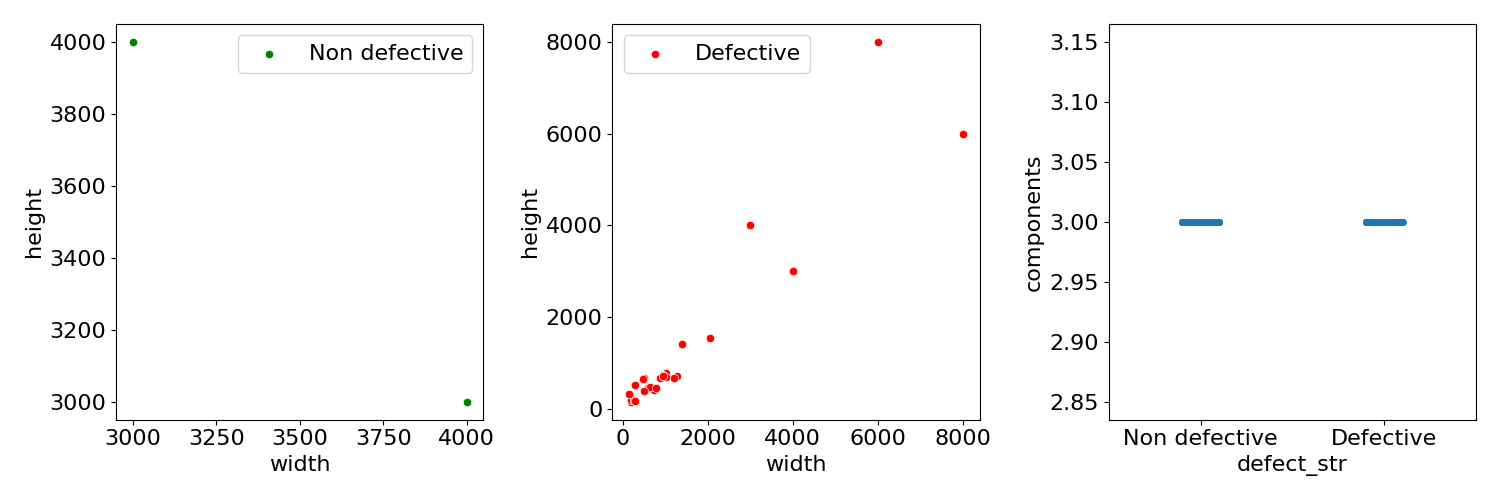
\includegraphics[width=\textwidth]{./tex_graphs/shapes.png}
	\caption{Distribution of the image shapes}
	\label{fig:shape_dist}
\end{figure}

Non defective pictures have only 2 shapes, either 3000x4000 or 4000x3000, depending whether it has
portrait or landscape orientation.
Defective images have wider distribution in the shapes reaching as high as 8000 pixels and as low as 148 pixels.
The minimum image size in this case is 148x194 (height x width) and the maximum is 8000x6000.
All images have 3 color components according to RGB color model.
However a differentiation based on the image shape might no be wise as it is missing any content related information.
A new image taken with different resolution might lead to improper prediction in the end.
The spread over the sizes indicate that during image processing if resizing is considered than not only
downscaling but upscaling might be necessary.

The distribution and correlation of the mean of the color components with respect to the images is shown on
Figure \ref{fig:comp_pair}.
\begin{figure}[!ht]
	\centering
	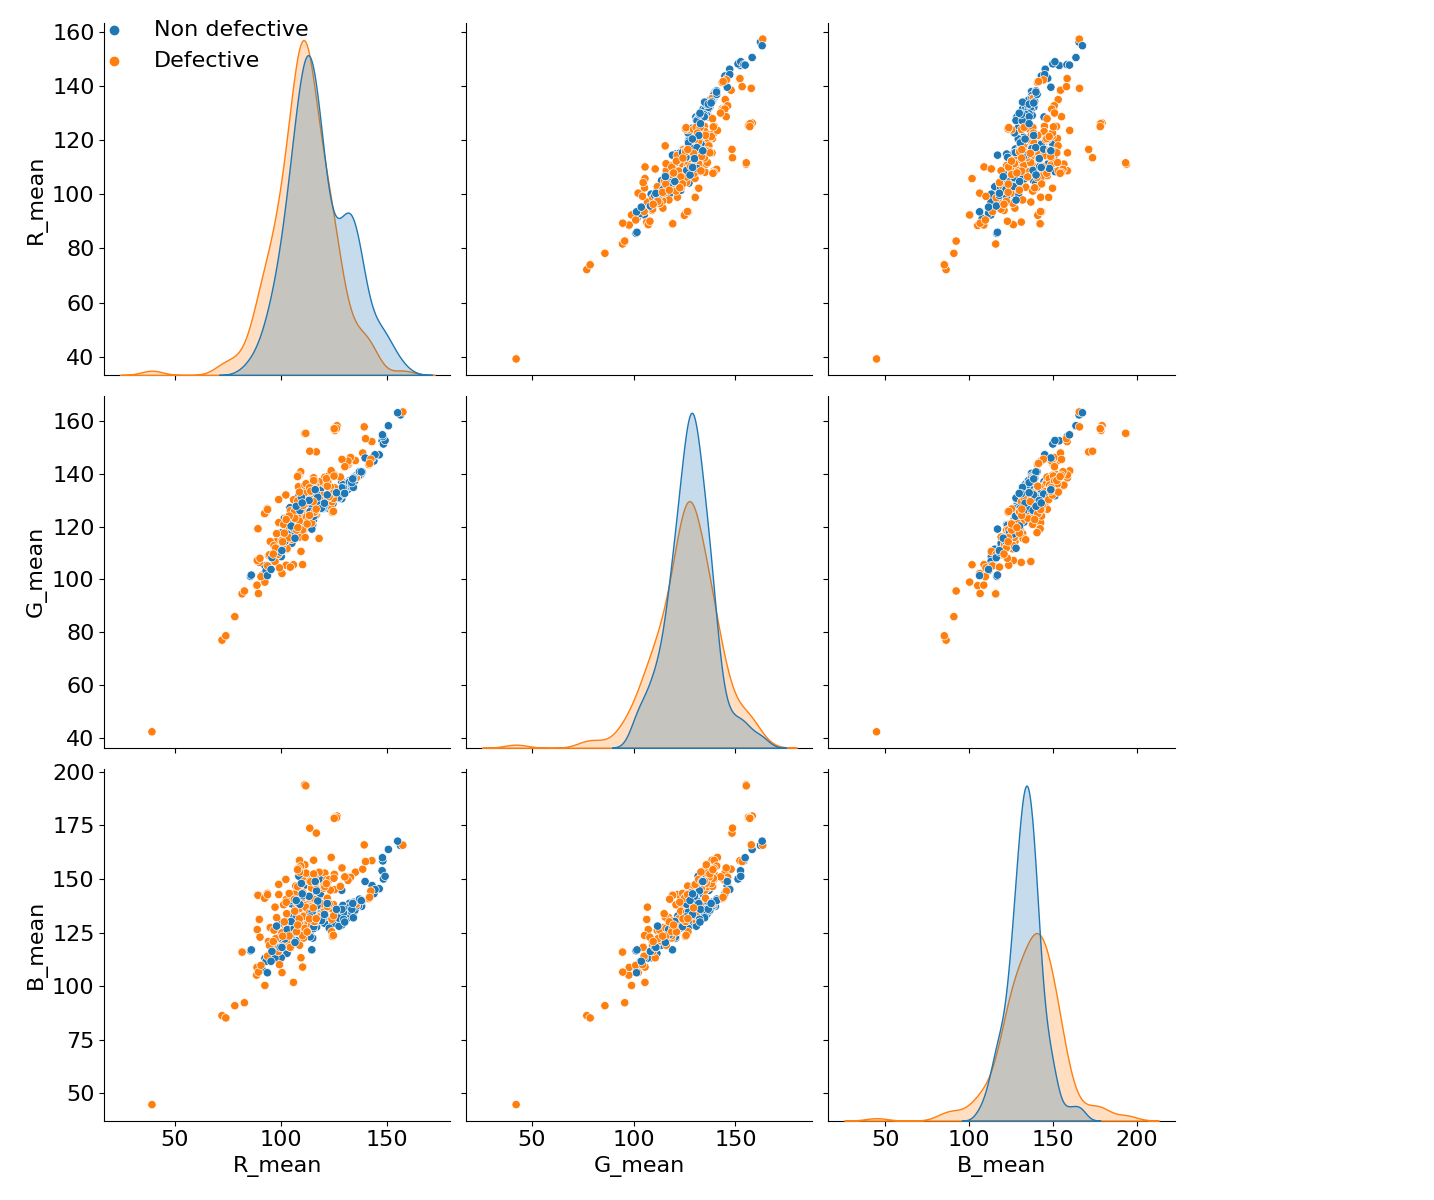
\includegraphics[width=\textwidth]{./tex_graphs/comp_pair.png}
	\caption{Color component pair analysis}
	\label{fig:comp_pair}
\end{figure}

The different color components show comparable histograms.
The case of the green and blue component the non defective components show a more narrow distribution.
The paired color components in both classes represent similar feature spaces.
Out of this no clear differentiation between defective and non defective classes can be done based on the color components.

During the study of the random samples, the following defects have been identified.
\begin{enumerate}
	\item Rail cracks. (Figure \ref{fig:def_cracked})
	\item Disjoint rail connections. (Figure \ref{fig:def_disjoint})
	\item Pitting of the rail surface. (Figure \ref{fig:def_pitting})
	\item Defect fastener. (Figure \ref{fig:def_nofix})
	\item Missing elements, e.g.: screws, springs. (Figure \ref{fig:def_missing})
\end{enumerate}
\begin{figure}[!ht]
	\centering
	\begin{subfigure}{0.3\textwidth}
		\centering
		\includegraphics[width=\textwidth]{./data/Train/Defective/287.jpg}
		\caption{Cracked rail}
		\label{fig:def_cracked}
	\end{subfigure}
	\begin{subfigure}{0.3\textwidth}
		\centering
		\includegraphics[width=\textwidth]{./data/Train/Defective/267.jpg}
		\caption{Disjoint rails}
		\label{fig:def_disjoint}
	\end{subfigure}
	\begin{subfigure}{0.3\textwidth}
		\centering
		\includegraphics[width=\textwidth]{./data/Train/Defective/260.jpg}
		\caption{Surface pitting}
		\label{fig:def_pitting}
	\end{subfigure}
	\begin{subfigure}{0.3\textwidth}
		\centering
		\includegraphics[width=\textwidth]{./data/Train/Defective/202.jpg}
		\caption{Fastener defect}
		\label{fig:def_nofix}
	\end{subfigure}
	\begin{subfigure}{0.3\textwidth}
		\centering
		\includegraphics[width=\textwidth]{./data/Train/Defective/215.jpg}
		\caption{Missing element}
		\label{fig:def_missing}
	\end{subfigure}
	\caption{Identified rail defects}
\end{figure}

The magnitude of each defect is varying in a wide range.
For example in case of cracked rails, from a crack of a few millimeters up to a missing rail part of several
centimeters can be found.
Similarly, surface pitting can range from small cracks on the surface up to severe cases, like shown in
Figure \ref{fig:def_pitting}.
In several cases components are missing that can be screws, fastening hooks or similar.
There are cases when these components are covered with ballast rocks.

\begin{figure}[!ht]
	\centering
	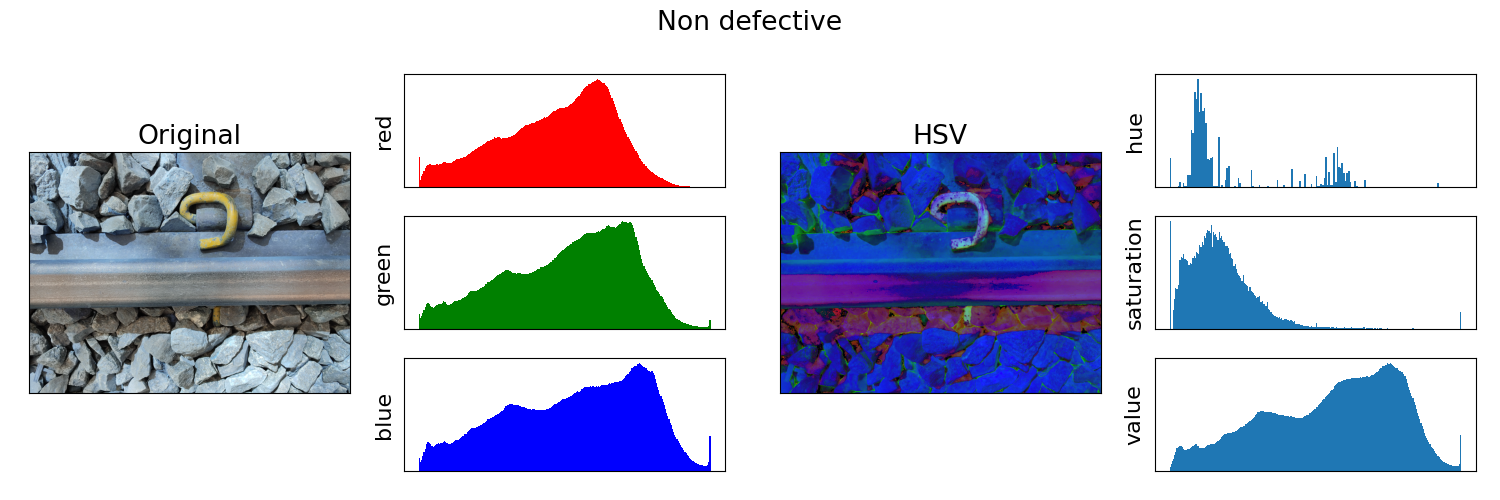
\includegraphics[width=0.8\textwidth]{./tex_graphs/comp_analysis_1.png}
	\caption{Color component analysis on RGB and HSV color modes}
	\label{fig:color_analysis}
\end{figure}

The color component analysis on RGB and HSV colormodes revealed no exact differentiation between the classes.
The component values highly depend on what is represented on the picture and how the photo is taken.
For example, presence of shadow has a significant impact on the component histogram.
An example of the analysis is shown on Figure \ref{fig:color_analysis}.
These histograms are taken for the overall picture, that is sorting every pixel into bins depending on their color values.

\begin{figure}[!ht]
	\centering
	\begin{subfigure}{0.3\textwidth}
		\centering
		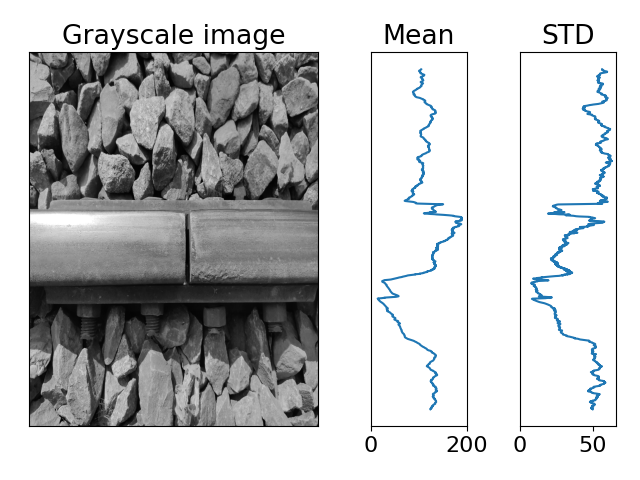
\includegraphics[width=\textwidth]{./tex_graphs/rail_surf_gray.png}
		\caption{Grayscale analysis}
		\label{fig:rail_surf_gray}
	\end{subfigure}
	\begin{subfigure}{0.3\textwidth}
		\centering
		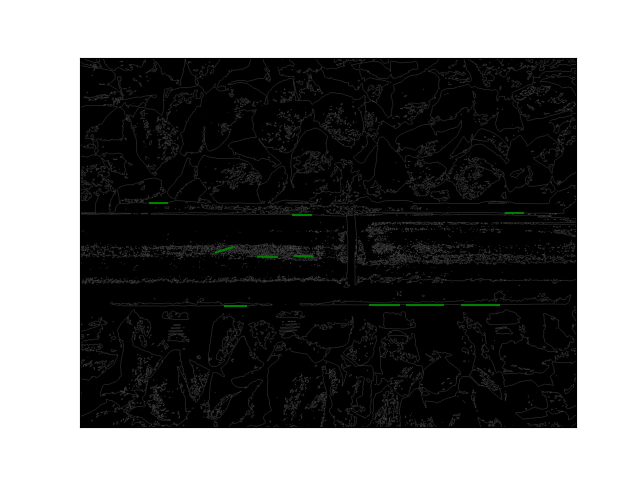
\includegraphics[width=\textwidth]{./tex_graphs/rail_surf_edge.png}
		\caption{Edge detection}
		\label{fig:rail_surf_edge}
	\end{subfigure}
	\begin{subfigure}{0.3\textwidth}
		\centering
		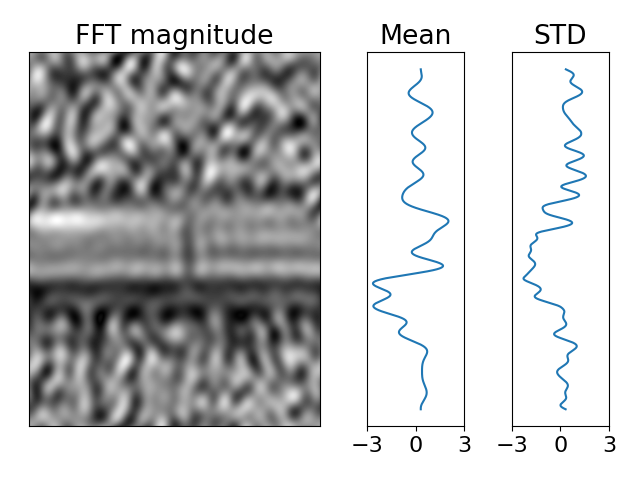
\includegraphics[width=\textwidth]{./tex_graphs/rail_surf_fft.png}
		\caption{FFT based detection}
		\label{fig:rail_surf_fft}
	\end{subfigure}
	\caption{Rail surface recognition}
\end{figure}

The grayscale analysis makes it possible to recognize rail surface as mentioned before.
The standard deviation and the mean value of the grayscale values correspond to the surface.
In cases when the rail orientation is alongside with the rows or columns, the identification is relatively easy.
If the means and standard deviations of the grayscale values are calculated row or columnwise, the resulting function
will bear the characteristics of the rail surface.
This is indicated on Figure \ref{fig:rail_surf_gray}.

In similar cases the edge detection works quite efficiently as the rail itself bears a couple of well-defined edges.
This makes it possible to detect line segments on the edge map which allows to detect the orientation of the rails.
Once this is known, the image can be rotated in an angle that the longitudinal position of the rail will be
perpendicular to the calculation direction as shown in Figure \ref{fig:rail_surf_edge}.
This allows the easy detection of the rail edges and makes the line detection (based on the Hough probability tansform)
very robust as indicated with the green sections that show the longest lines detected.
The surface detection can be improved by applying a FFT transform to the image and standardising the mean and
standard deviation values.
Such composition is shown on Figure \ref{fig:rail_surf_fft}.

Due to the high variety of the image content (as shown in Figure \ref{fig:variety}),
orientation and defect method none of the mentioned algorithm lead to a clear segmentation of the image.
This prevents the localization of any classification algorithm and also prevents the application of any approach that
is mentioned in Section \ref{sec:intro}.
To cope with the classification task we turn then to CNNs.

\begin{figure}[!ht]
	\centering
	\begin{subfigure}{0.3\textwidth}
		\centering
		\includegraphics[width=\textwidth]{./data/Train/Defective/162.jpg}
	\end{subfigure}
	\begin{subfigure}{0.3\textwidth}
		\centering
		\includegraphics[width=\textwidth]{./data/Train/Defective/224.jpg}
	\end{subfigure}
	\begin{subfigure}{0.3\textwidth}
		\centering
		\includegraphics[width=\textwidth]{./data/Train/Non defective/2.jpg}
	\end{subfigure}
	\caption{Variety of dataset}
	\label{fig:variety}
\end{figure}

\subsection{LeNet-5} \label{sec:Lenet5}
LeNet-5 is one of the earliest models used originally for the handwritten digit recogniton.
It suffers from computational limitations due to the low performance of the computers at the time of being constructed,
but it defined the basic structure of a convolutional networks used afterwads.
The structure of the neural network according to Tensorflow Keras is shown in Table \ref{table:LeNet5_struct}.
As the input is limited to a single channel, the images were converted to grayscale followed by adaptive histogram
normalization (CLAHE) and noise filtering with a median filter with kernel of 11x11.
After all the changes applied, the images were resized to 32x32 pixels.

\begin{table}[!ht]
	\centering
	\begin{tabular}{l c c c c c c}
		Layer            & Filters / Neurons & Size / Rate & Padding & Stride & Feature map  & Activation \\
		\hline
		Input            & -                 & -           & -       & -      & 32 x 32 x 1  & -          \\
		Rescaling        & -                 & -           & -       & -      & 32 x 32 x 1  & -          \\
		Conv2D           & 6                 & 5 x 5       & valid   & 2      & 28 x 28 x 6  & tanh       \\
		AveragePooling2D & -                 & 2 x 2       & -       & 1      & 14 x 14 x 6  & -          \\
		Conv2D           & 16                & 5 x 5       & valid   & 2      & 10 x 10 x 16 & tanh       \\
		AveragePooling2D & -                 & 2 x 2       & -       & 1      & 5 x 5 x 16   & -          \\
		Flatten          & -                 & -           & -       & -      & 400          & -          \\
		Dense            & 120               & -           & -       & -      & 120          & tanh       \\
		Dense            & 84                & -           & -       & -      & 84           & tanh       \\
		Dense            & 1                 & -           & -       & -      & 1            & sigmoid    \\
		\hline
	\end{tabular}
	\caption{LeNet-5 layer structure}
	\label{table:LeNet5_struct}
\end{table}

A learning rate of 0.0001 was used as initial value which was decreased by the ReduceLROnPlateau callback to 0.000005 by
a factor of 0.5 and with a patience set to 2.
The accuracy peak on the validation dataset reached with a low number of epochs.
The resulting metrics are shown in \ref{fig:LeNet5_metrics}.

\begin{figure}[!ht]
	\centering
	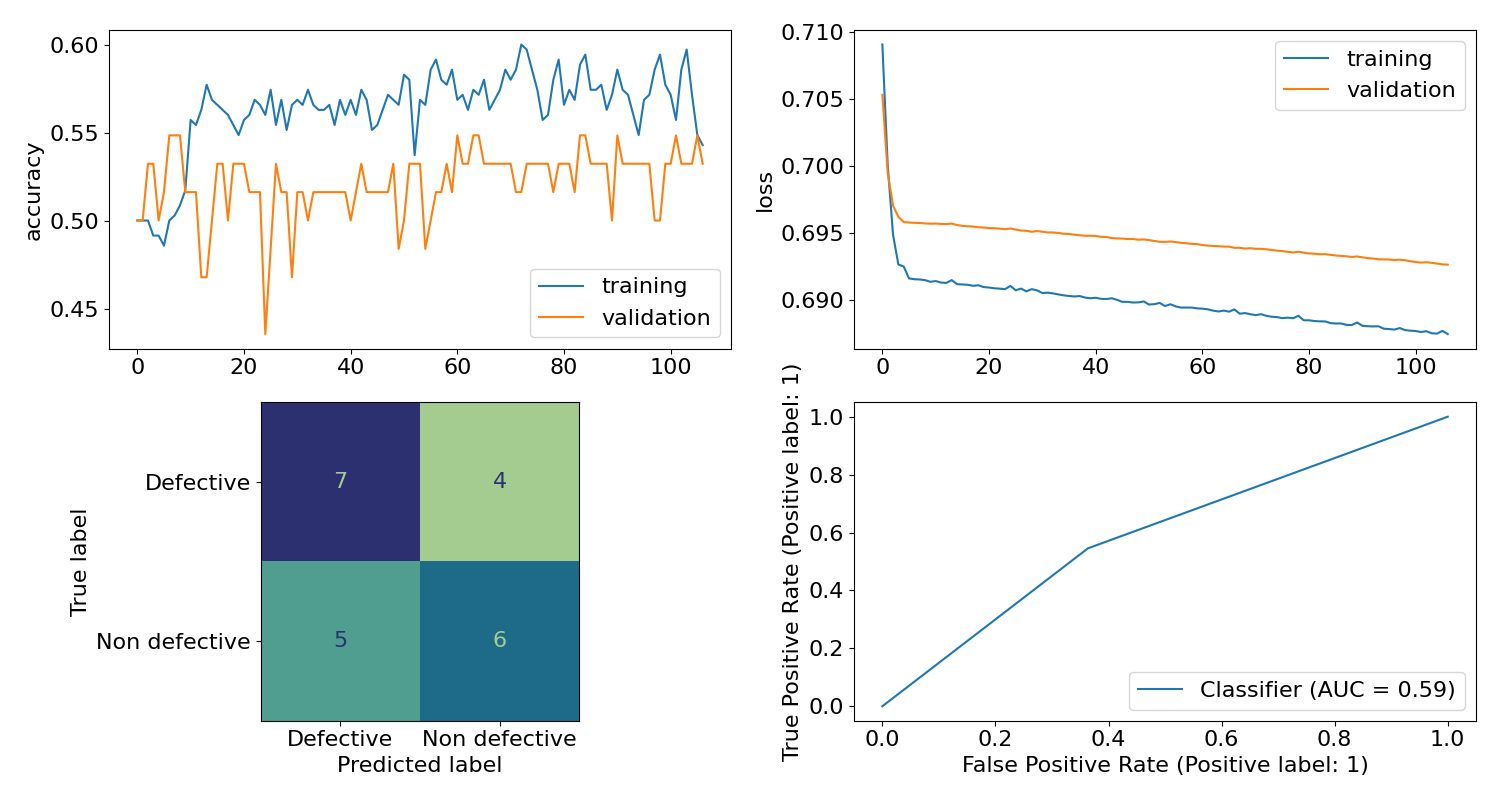
\includegraphics[width=\textwidth]{./tex_graphs/metrics_LeNet-5.png}
	\caption{LeNet-5 metrics}
	\label{fig:LeNet5_metrics}
\end{figure}

The accuracy increases rapidly in teh first few epochs topping at around the 10th epoch at 59.67\% on the
validation dataset.
Afterwards the training accuracy slightly decreases and the validation accuracy decreases as well.
The latter is showing bigger fluctuation, mostly due to the limited number of validation data points, a single
change in the classification in one of the images leaves to a bigger relative change.
The loss function decreases continuously for both datasets, howevere an increasing distance between the two
is observed.
The confusion matrix and the ROC curve shows a classifier with 59\% accuracy.
However a deeper look into the learning curves reveal that the increasing gap between the training and validation
data shows that the training data might be unrepresentative to the test data.
It has to be noted that for different training sessions the confusion matrix and ROC curve also show some
variance of accuracy ranging down to 45\%.
The resulting trained model did not prove to be stable.
This could be due to the fact that the layer structure is very limited and failed to learn the proper features
or the training data is not representative to the test data.

\subsection{AlexNet} \label{sec:AlexNet}
AlexNet is the second major convolutional network borught up several years after LeNet-5 was introduced.
Compared to LeNet-5 it's depth, width and resolution is increased significantly.
The structure is described in Table \ref{table:AlexNet_struct}.
It introduces ReLU activation function together with DropOut layers and overlapping pooling.
The input accepts color pictures, therefore no manipulation of the images were done, except resizing to
correct size.

\begin{table}[!ht]
	\centering
	\begin{tabular}{l c c c c c c}
		Layer        & Filters / Neurons & Size / Rate & Padding & Stride & Feature map   & Activation \\
		\hline
		Input        & -                 & -           & -       & -      & 227 x 227 x 3 & -          \\
		Rescaling    & -                 & -           & -       & -      & 227 x 227 x 3 & -          \\
		Conv2D       & 96                & 11 x 11     & valid   & 4      & 55 x 55 x 96  & ReLU       \\
		MaxPooling2D & -                 & 3 x 3       & valid   & 2      & 27 x 27 x 96  & -          \\
		Conv2D       & 256               & 5 x 5       & same    & 1      & 27 x 27 x 256 & ReLU       \\
		MaxPooling2D & -                 & 3 x 3       & valid   & 2      & 13 x 13 x 256 & -          \\
		Conv2D       & 384               & 3 x 3       & same    & 1      & 13 x 13 x 384 & ReLU       \\
		Conv2D       & 384               & 3 x 3       & same    & 1      & 13 x 13 x 384 & ReLU       \\
		Conv2D       & 256               & 3 x 3       & same    & 1      & 13 x 13 x 256 & ReLU       \\
		MaxPooling2D & -                 & 3 x 3       & valid   & 2      & 6 x 6 x 256   & -          \\
		Dropout      & -                 & 0.5         & -       & -      & 6 x 6 x 256   & -          \\
		Flatten      & -                 & -           & -       & -      & 9216          & -          \\
		Dense        & 4096              & -           & -       & -      & 4096          & ReLU       \\
		Dropout      & -                 & 0.5         & -       & -      & 4096          & -          \\
		Dense        & 4096              & -           & -       & -      & 4096          & ReLU       \\
		Dense        & 1                 & -           & -       & -      & 1             & sigmoid    \\
		\hline
	\end{tabular}
	\caption{AlexNet layer structure}
	\label{table:AlexNet_struct}
\end{table}

During training the same optimization settings were applied as for LeNet-5.
The training time increased significantly due to the increase of the trainable parameters.
The results are shown in Figure \ref{fig:AlexNet_metrics}.

\begin{figure}[!ht]
	\centering
	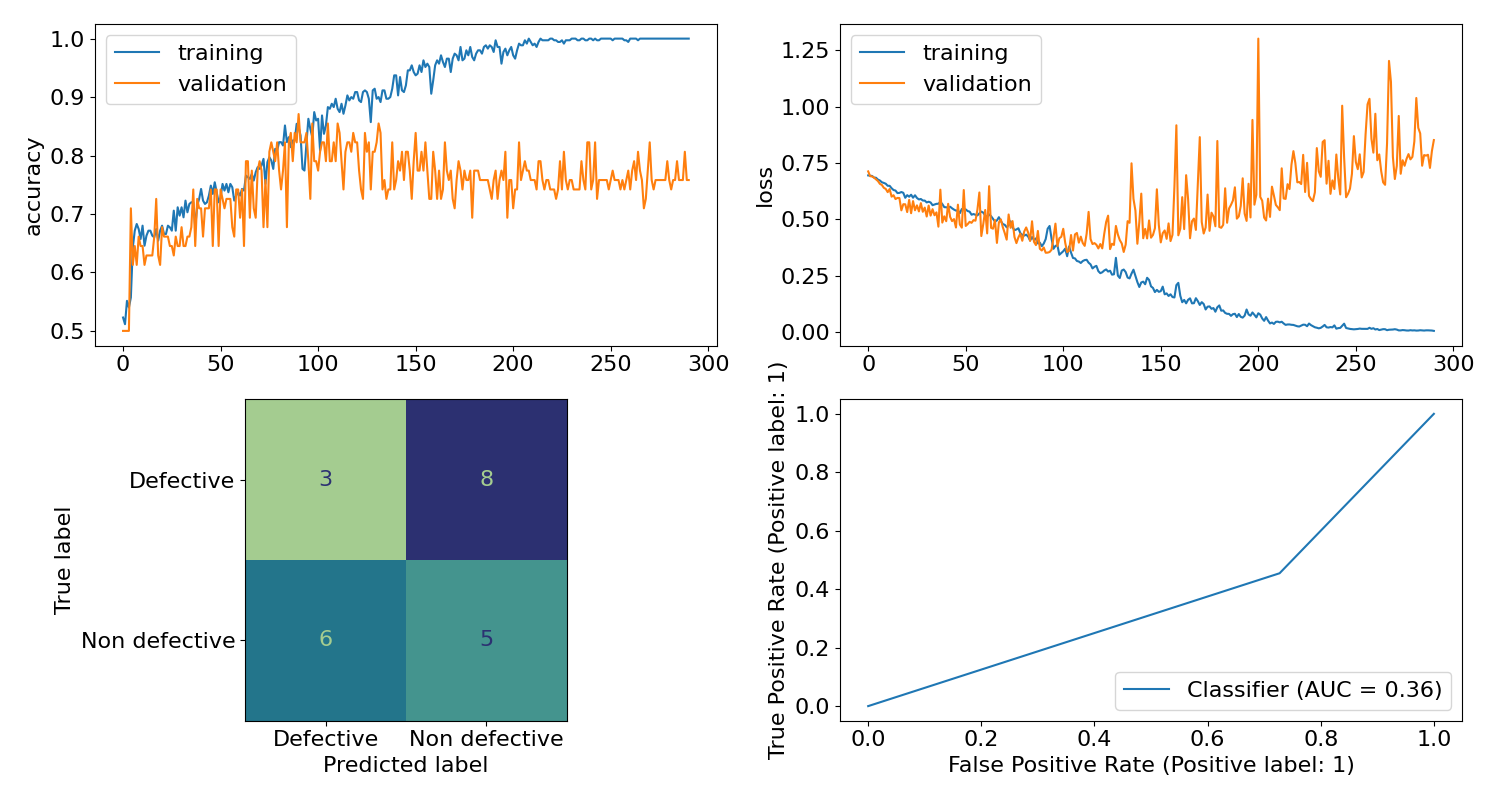
\includegraphics[width=\textwidth]{./tex_graphs/metrics_AlexNet.png}
	\caption{AlexNet metrics}
	\label{fig:AlexNet_metrics}
\end{figure}

An accuracy rate of 87\% achieved on the validation dataset, whilst the training accuracy reaches 100\%.
This indicates that the network is able to learn the training dataset, but an overfitting can be seen after
approx. 120 epochs.
Same can be seen on the learning curves as well.
The confusion matrix understates that the training data is not representative to the test data.
A fairly good fitting validation set did not result in a good fit on the test data, only an accuracy of
36 \% achieved.

\subsection{VGG16} \label{sec:VGG16}
The VGG model brings a different approach to the structure of the CNNs.
Instead of using single big filters (like a 11 x 11 filter in AlexNet), several smaller filters applied
consecutevily.
Applying such small filter on the input layer results in a larger feature map on the input.
Additionally increasing the number of consecutive layers reduce the tendency to overfit.
The implemented structure of VGG16 is shown on Table \ref{table:VGG16_struct}.
As input image, resized color images used without any further alteration.

\begin{table}[!ht]
	\centering
	\begin{tabular}{l c c c c c c}
		Layer        & Filters / Neurons & Size / Rate & Padding & Stride & Feature map     & Activation \\
		\hline
		Input        & -                 & -           & -       & -      & 224 x 224 x 3   & -          \\
		Rescaling    & -                 & -           & -       & -      & 224 x 224 x 3   & -          \\
		Conv2D       & 64                & 3 x 3       & same    & 1      & 224 x 224 x 64  & ReLU       \\
		Conv2D       & 64                & 3 x 3       & same    & 1      & 224 x 224 x 64  & ReLU       \\
		MaxPooling2D & -                 & 2 x 2       & valid   & 2      & 112 x 112 x 64  & -          \\
		Conv2D       & 128               & 3 x 3       & same    & 1      & 112 x 112 x 128 & ReLU       \\
		Conv2D       & 128               & 3 x 3       & same    & 1      & 112 x 112 x 128 & ReLU       \\
		MaxPooling2D & -                 & 2 x 2       & valid   & 2      & 56 x 56 x 128   & -          \\
		Conv2D       & 256               & 3 x 3       & same    & 1      & 56 x 56 x 256   & ReLU       \\
		Conv2D       & 256               & 3 x 3       & same    & 1      & 56 x 56 x 256   & ReLU       \\
		Conv2D       & 256               & 3 x 3       & same    & 1      & 56 x 56 x 256   & ReLU       \\
		MaxPooling2D & -                 & 2 x 2       & valid   & 2      & 28 x 28 x 256   & -          \\
		Conv2D       & 512               & 3 x 3       & same    & 1      & 28 x 28 x 512   & ReLU       \\
		Conv2D       & 512               & 3 x 3       & same    & 1      & 28 x 28 x 512   & ReLU       \\
		Conv2D       & 512               & 3 x 3       & same    & 1      & 28 x 28 x 512   & ReLU       \\
		MaxPooling2D & -                 & 2 x 2       & valid   & 2      & 14 x 14 x 512   & -          \\
		Conv2D       & 512               & 3 x 3       & same    & 1      & 14 x 14 x 512   & ReLU       \\
		Conv2D       & 512               & 3 x 3       & same    & 1      & 14 x 14 x 512   & ReLU       \\
		Conv2D       & 512               & 3 x 3       & same    & 1      & 14 x 14 x 512   & ReLU       \\
		MaxPooling2D & -                 & 2 x 2       & valid   & 2      & 7 x 7 x 512     & -          \\
		Flatten      & -                 & -           & -       & -      & 25088           & -          \\
		Dense        & 4096              & -           & -       & -      & 4096            & ReLU       \\
		Dense        & 4096              & -           & -       & -      & 4096            & ReLU       \\
		Dense        & 1                 & -           & -       & -      & 1               & sigmoid    \\
		\hline
	\end{tabular}
	\caption{VGG16 layer structure}
	\label{table:VGG16_struct}
\end{table}

The initial learning rate is reduced to 0.00001 and the ReduceLROnPlateau patience was set to 1.
This helped to found the local minimum only in a few starting epochs.
This model required the longest training time.
The resulting metrics can be seen on Figure \ref{fig:VGG16_metrics}.

\begin{figure}[!ht]
	\centering
	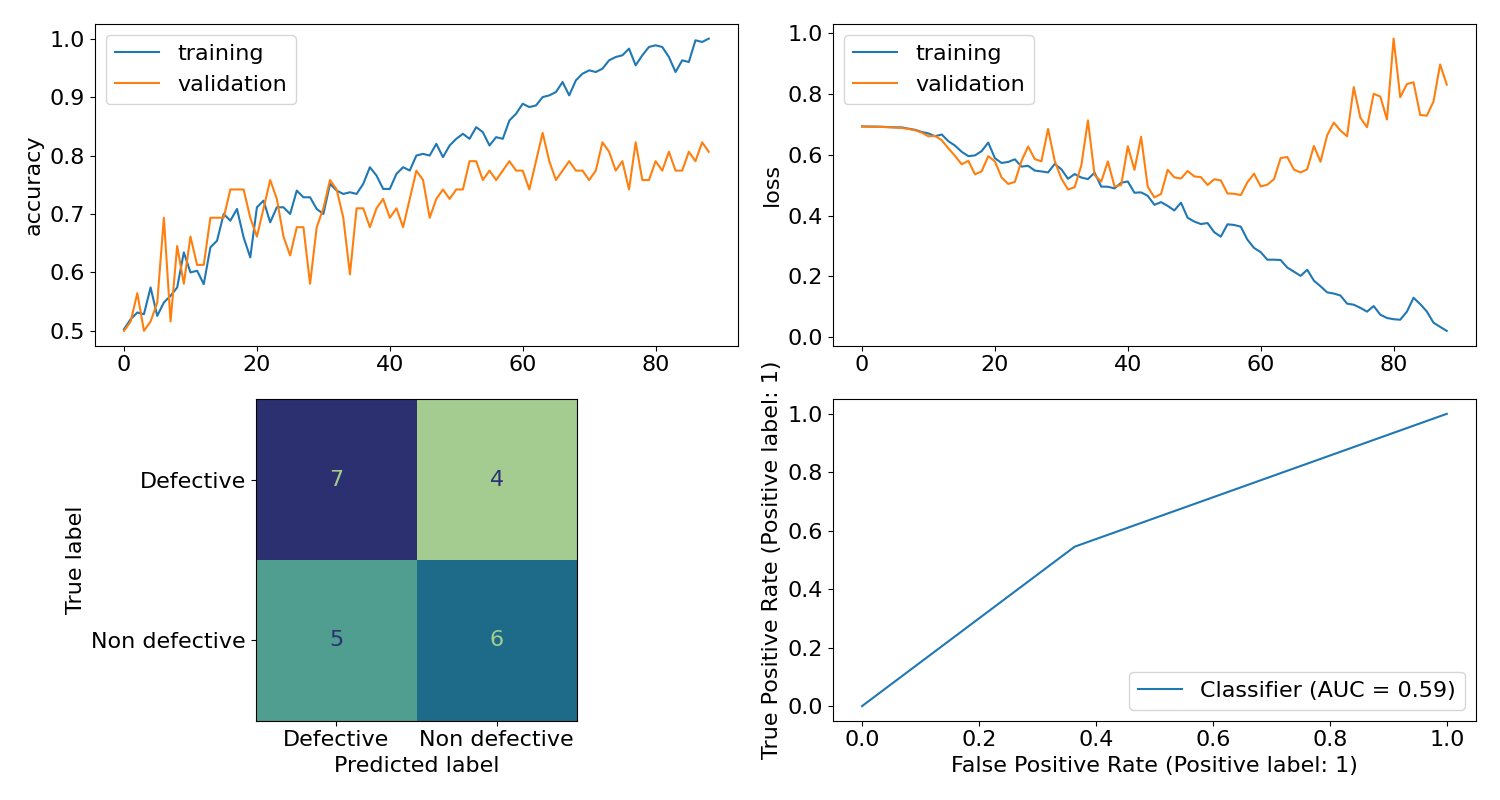
\includegraphics[width=\textwidth]{./tex_graphs/metrics_VGG16.png}
	\caption{VGG16 metrics}
	\label{fig:VGG16_metrics}
\end{figure}

The training needed much less epochs than in previous case, reaching the validation accuracy of 83.87\% at the
64\textsuperscript{th} eopch.
An overfitting can be seen from the learning curve, which indicates optimal epoch number of 45, where the
validation accuracy was 77.41\%.
The model fitted to the test data resulting in an accuracy of 59\%, although due to long running time only a single
training is performed, therefore the assumption that the training data is not representative to the test data
can not be dropped.

\subsection{Pretrained VGG16}
In order to improve our models, pretrained models are applied.
To allow comparison on the effect of prelearned features the same VGG16 model was selected.
An initial learning rate  is set to 0.00001 with a ReduceLROnPlateau callback set with a patience of 1 and minimal
learning rate of 0.000001.

\begin{figure}[!ht]
	\centering
	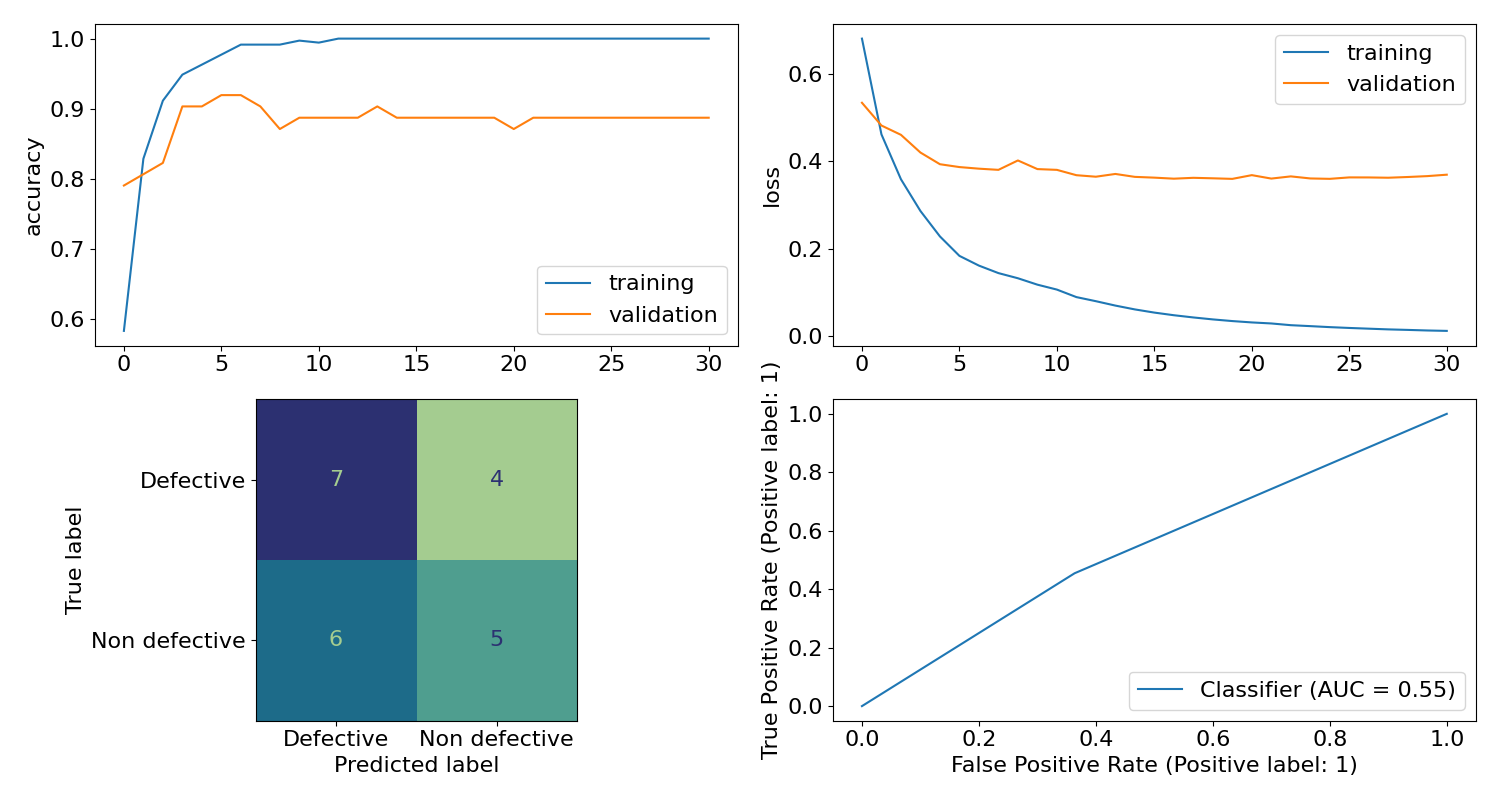
\includegraphics[width=\textwidth]{./tex_graphs/metrics_VGG16_pretrained.png}
	\caption{Pretrained VGG16 metrics}
	\label{fig:VGG16_pretrained_metrics}
\end{figure}

The model shows significant improvement in the performance the top accuracy of 91.93\% is reached after 6 epochs
on the validation set.
The unrepresentativeness of the training data can be observed slightly on the learning curves after approximately
10 epochs.
The test data shows a classifier with an accuracy of 59\%.
During fine-tuning both the initial and the minimal learning rate was reduced to the one tenth.
Unfortunately no improvement to the model achieved.

\subsection{Pretrained ResNet50}
Second pretrained model used is the ResNet50 that applies fewer filters with lower complexity.
Shortcut connections added between sets of convolutional layers to perform identity mapping.

The training with feature extraction settings done with an initial learning rate of 0.0001 and a minimum learning
rate of 0.000005 added with ReduceLROnPlateau.

\begin{figure}[!ht]
	\centering
	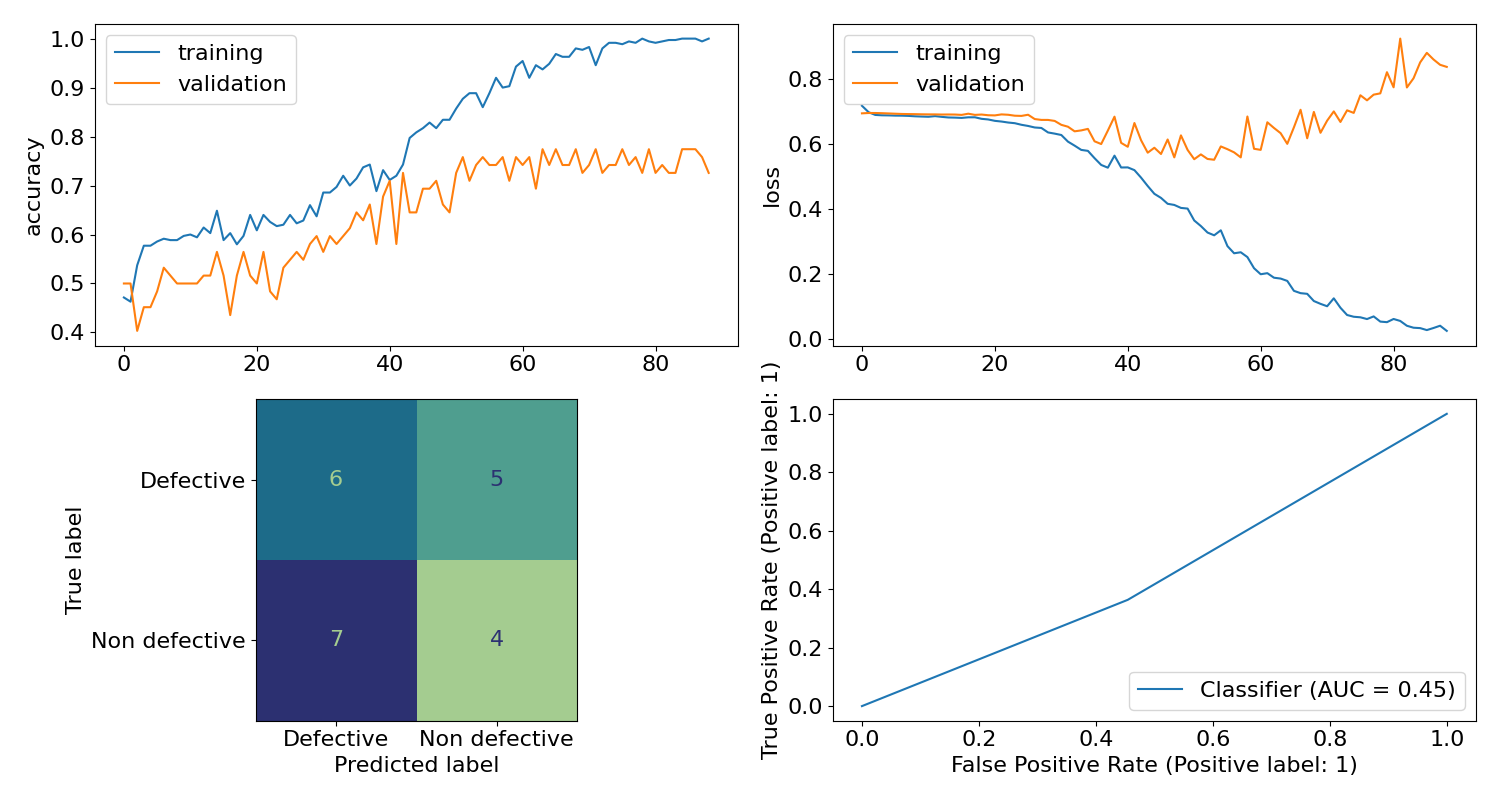
\includegraphics[width=\textwidth]{./tex_graphs/metrics_ResNet50_pretrained.png}
	\caption{Pretrained ResNet50 metrics}
	\label{fig:ResNet50_pretrained_metrics}
\end{figure}

The model performed fairl well reaching an accuracy rate 64.51\% on the validation set.
The loss function of the validation set is lower than of the training set indicating that the model was fitted
better on the validation set than to the training set.
This might happend due to regulraization applied during training, low size of validation set, the validation set
is not representative to the training set or due to the applied data augmentation.
In our case all of the above (except the regularization) might contribute to this effect.

\begin{figure}[!ht]
	\centering
	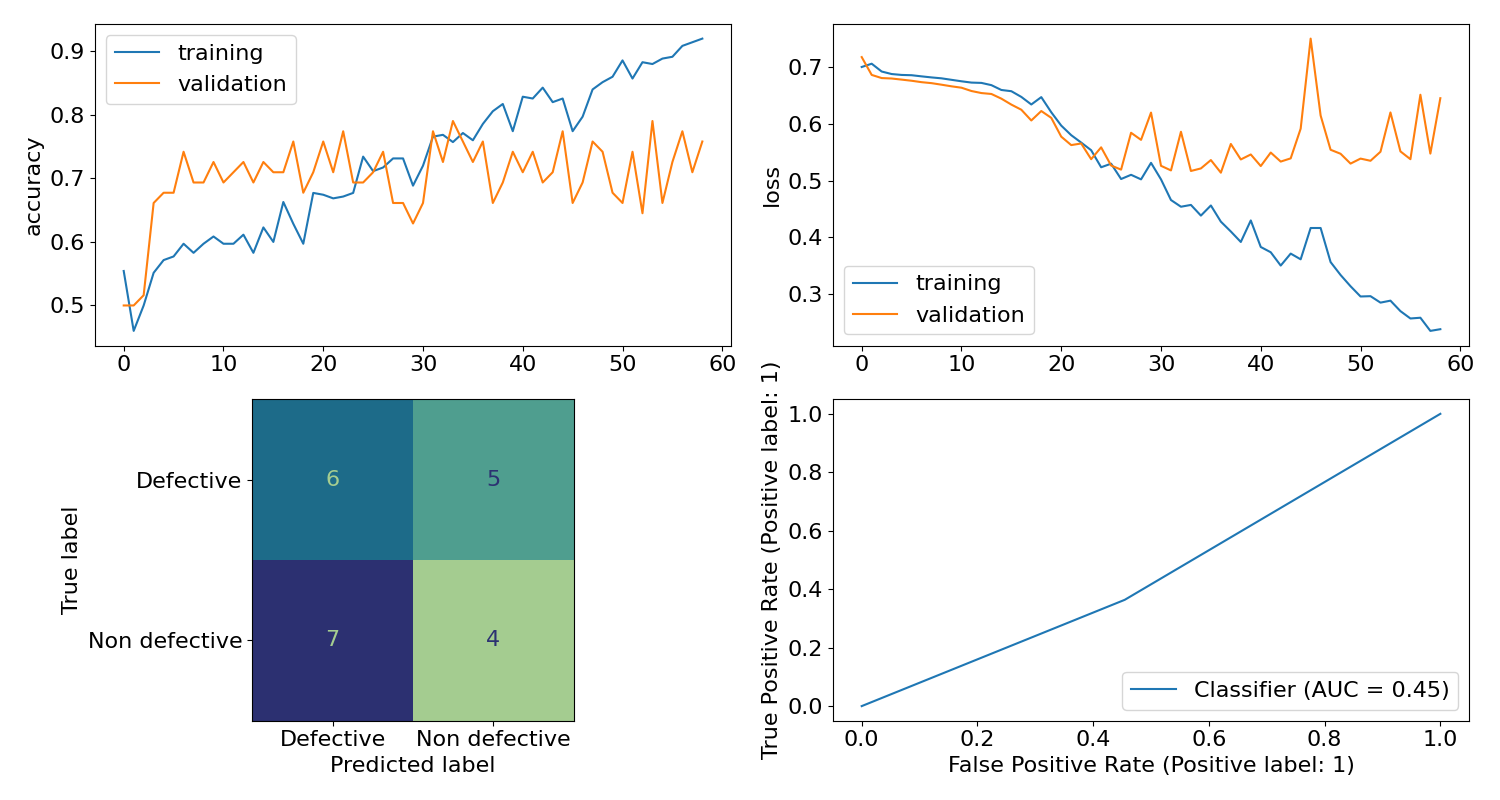
\includegraphics[width=\textwidth]{./tex_graphs/metrics_ResNet50_pretrained_finetuned.png}
	\caption{Fine-tuned ResNet50 metrics}
	\label{fig:ResNet50_finetuned_metrics}
\end{figure}

Applying fine-tuning by reducing the learning rates to the one tenth resulted in a siginificatn improvement
of the model performance.
The accuracy on validation set reached 79.03\%.
However the unrepresentative train dataset can be once again observed on the learning curves.
For both results (feature extraction only and fine tuning applied) the classifier performed poorly on the test
dataset with 41\% and 45\% accuracy rates respectively.

\section{Discussion} \label{sec:discussion}
The results of the applied models are summarized in Table \ref{table:results_summary}.
Two major observations present, from one side the model performance highly depends on the selected learning rate,
and on the other side the representativeness between test and training dataset needs to be checked more in detail.
To address these two points further tuning of the models done by applying a random search algorithm on the learning rates
and performing resampling to assess the accuracy rates better.

\begin{table}[!ht]
	\centering
	\begin{tabular}{l c c c c c}
		\multirow{2}{*}{Model} & \multicolumn{2}{c}{Training} & \multicolumn{2}{c}{Validation} & \multirow{2}{*}{Test Accuracy}                 \\
		                       & Accuracy                     & Loss                           & Accuracy                       & Loss   &      \\
		\hline
		LeNet-5                & 59.14\%                      & 0.6858                         & 59.68\%                        & 0.6884 & 59\% \\
		AlexNet                & 84.86\%                      & 0.3921                         & 87.10\%                        & 0.3749 & 36\% \\
		VGG16                  & 90.00\%                      & 0.2541                         & 83.87\%                        & 0.5895 & 59\% \\
		Pretrained VGG16       & 97.71\%                      & 0.1840                         & 91.94\%                        & 0.3871 & 55\% \\
		Pretrained ResNet50    & 48.86\%                      & 0.6936                         & 64.52\%                        & 0.6836 & 41\% \\
		Fine-tuned ResNet50    & 75.71\%                      & 0.4569                         & 79.03\%                        & 0.5169 & 45\% \\
		\hline
	\end{tabular}
	\caption{Model results at optimal number of epochs}
	\label{table:results_summary}
\end{table}

A deeper look into the test dataset reveals a possible root cause of the unrepresentativity issue.
Figure \ref{fig:unrepr_test} shows the image that is part of the test data and shows basically the same image to be classified.
Furthermore this particular image is not an easily understandable case for the model, it is a very specific track failure with
very limited comparable image in the training dataset.
A misclassification of these images could lead to a test accuracy deviation of 13.64\%.
The test and validation accuracy is comparable only in case of the LeNet-5.
The other models show much higher deviation between these two metrics than 13.64\%, therefore this might be not the only reason.

\begin{figure}[!ht]
	\centering
	\begin{subfigure}{0.3\textwidth}
		\centering
		\includegraphics[width=\textwidth]{./data/Test/Defective/374.jpg}
	\end{subfigure}
	\begin{subfigure}{0.3\textwidth}
		\centering
		\includegraphics[width=\textwidth]{./data/Test/Defective/375.jpg}
	\end{subfigure}
	\begin{subfigure}{0.3\textwidth}
		\centering
		\includegraphics[width=\textwidth]{./data/Test/Defective/381.jpg}
	\end{subfigure}
	\caption{Unrepresentative samples from test dataset}
	\label{fig:unrepr_test}
\end{figure}

\subsection{Fine tuning of learning rates}
Initially the learning rates were manually selected and the ReduceLROnPlateau callback was applied.
Due to the fact that the size of the validation dataset is very limited, the classification of a single image leads
to an change of 1.6\% in terms of validation accuracy.
In case the value of the learning rate is set to too low, several epochs need to be run to achieve a change in the
validationa accuracy score.
Therefore the chance that the ReduceLROnPlateau reduces further the learning rate is very high.
To avoid this behaviour, during fine tuning constant learning rate was applied.
To realize the random search the modul \lstinline{keras_tuner} was used.
This allows easy hypertuning of the parameters, that is realised in \lstinline{hp_tuner.ipynb}.
The range of learning rate was set to cover an interval one magnitude higher and one magnitude lower compared to the
manually selected learning rate.
The number of epochs was set to be at least as much as the optimal epoch number in the manual case and overall
10 randomly selected values were run.
In this way the accuracy rate of LeNet-5 and AlexNet was significantly improved, and the pretrained ResNet50 show some
improvement, however in latter case the final result after fine-tuning of the model did not lead to any further increase
in the validation accuracy.
The results are presented in Table, \ref{table:results_keras_tuner}, changes shown in red.

\begin{table}[!ht]
	\centering
	\begin{tabular}{l c c c c c}
		\multirow{2}{*}{Model} & \multicolumn{2}{c}{Training} & \multicolumn{2}{c}{Validation} & \multirow{2}{*}{Test Accuracy}                                             \\
		                       & Accuracy                     & Loss                           & Accuracy                       & Loss                 &                    \\
		\hline
		LeNet-5                & {\color{red} 60.00\%}        & {\color{red} 0.6842}           & {\color{red} 62.90\%}          & {\color{red} 0.6892} & 59\%               \\
		AlexNet                & {\color{red} 100.00\%}       & {\color{red} 0.0039}           & {\color{red} 91.94\%}          & {\color{red} 0.5422} & {\color{red} 45\%} \\
		VGG16                  & 90.00\%                      & 0.2541                         & 83.87\%                        & 0.5895               & 59\%               \\
		Pretrained VGG16       & {\color{red} 99.71\%}        & {\color{red} 0.1436}           & 91.94\%                        & {\color{red} 0.3830} & {\color{red} 23\%} \\
		Pretrained ResNet50    & {\color{red} 52.86\%}        & {\color{red} 0.6882}           & {\color{red} 74.19\%}          & {\color{red} 0.6734} & {\color{red} 45\%} \\
		Fine-tuned ResNet50    & 75.71\%                      & 0.4569                         & 79.03\%                        & 0.5169               & 45\%               \\
		\hline
	\end{tabular}
	\caption{Results after hypertuning the learning rates}
	\label{table:results_keras_tuner}
\end{table}

In case of simpler neural networks (LeNet-5, AlexNet) the tuning of the learning rate proved to be an efficient approach.
However in case of more deeper networks (VGG16, ResNet50) no significant improvement is achieved, except the pretrained ResNet50
prior to finetuning of the network parameters, that is considered as an intermediate status when building a CNN model.
The reason behind might be that a more sophisticated approach on learning rates is used during manual setup.
An adaptive setting might result in a situation when a local minimum can be approached much closer that in case of a constant learning
rate as the number of epochs was limited durin retraining the models with the hypertuned learning rate.
All in all, a few bigger steps in the beginning followed by a sequential lowering of the learning rate might be a more useful approach
for these networks.
Due to the limited computational capacity this is not investigated further in the scope of this study.

\subsection{Resampling}
In order to achieve a reliable performance indicator in terms of accuracy, resampling is advised, in this particular case bootstrapping
is used.
A custom function is defined to resample the datasets including the training, validation and test dataset.
In this way several dataset can be created and separate models can be trained for all of them.
This allows evaluating the single models on data that is not used for training at all, and furthermore allows to increase
the representativeness of the training data to the test data.
Once the single models are evaluated, the final metric is derived by taking the average of the test accuracies.

\section{Conclusion} \label{sec:conclusion}
\newpage
\listoffigures
\newpage
\listoftables
\newpage
\printbibliography
\end{document}